\documentclass{beamer}
\usepackage{amsmath}
\usepackage{listings}
\usepackage{listings}
\usepackage{floatflt}
\usepackage{qtree}
\lstset{language=Haskell,basicstyle=\ttfamily}
%\usepackage{beamerthemesplit}
\usetheme{Szeged}
 
\title{The Pairing Heap}
\subtitle{A Self-Adjusting Heap}
\author{Fredman et al}
\date{\today}
\newcommand{\bind}{\texttt{>>=}}
\newcommand{\ret}{\texttt{return}}
\newcommand{\bs}{\texttt{\char`\\}}
\newcommand{\fs}{\char`/}
\newcommand{\at}{\texttt{a}}
\newcommand{\kt}{\texttt{k}}
\newcommand{\mt}{\texttt{k}}
\begin{document}
\lstset{basicstyle=\footnotesize\ttfamily}
%\section*{Introduction}
\begin{frame}
  \titlepage
\end{frame}
 
\section{The Pairing Heap}
\subsection{}
\begin{frame}[fragile]
\frametitle{Pairing Heaps}

The pairing heap consists of a single heap-ordered multiway tree:\\

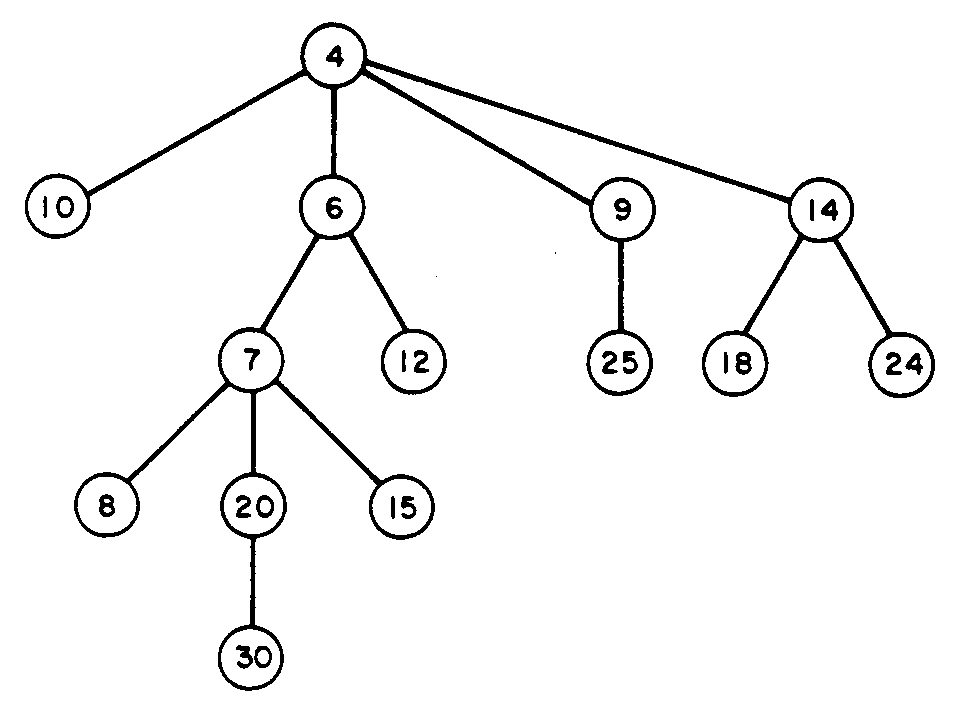
\includegraphics[width=7cm]{fig1.png}

\end{frame}

\begin{frame}
\frametitle{Linking}

Combine two heap-ordered trees by linking the smaller root to the larger root

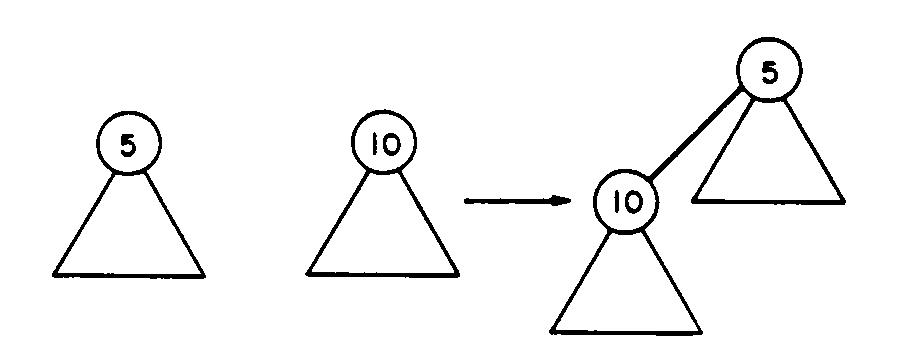
\includegraphics[width=7cm]{fig2.png}

\end{frame}
 
\begin{frame}
\frametitle{Heap operations}

\textbf{find-min}: Return the root of the tree

\textbf{insert $x$}: Make $x$ a one-node tree and link it with the heap tree

\textbf{meld}: Link the two heap trees and return the new tree

\textbf{decrease-key $x$}: Decrease the key of $x$. If $x$ is not the root cut
the subtree including $x$ and link it on the main tree.

\textbf{delete $x$}: If $x$ is the root, do \textbf{delete-min}. If not, cut $x$
and its subtree from the main tree, perform \textbf{delete-min} on $x$'s subtree
and link the result with the main tree.

\textbf{delete-min}: Non-trivial.

\end{frame}

\begin{frame}
\frametitle{Child, sibling representation}

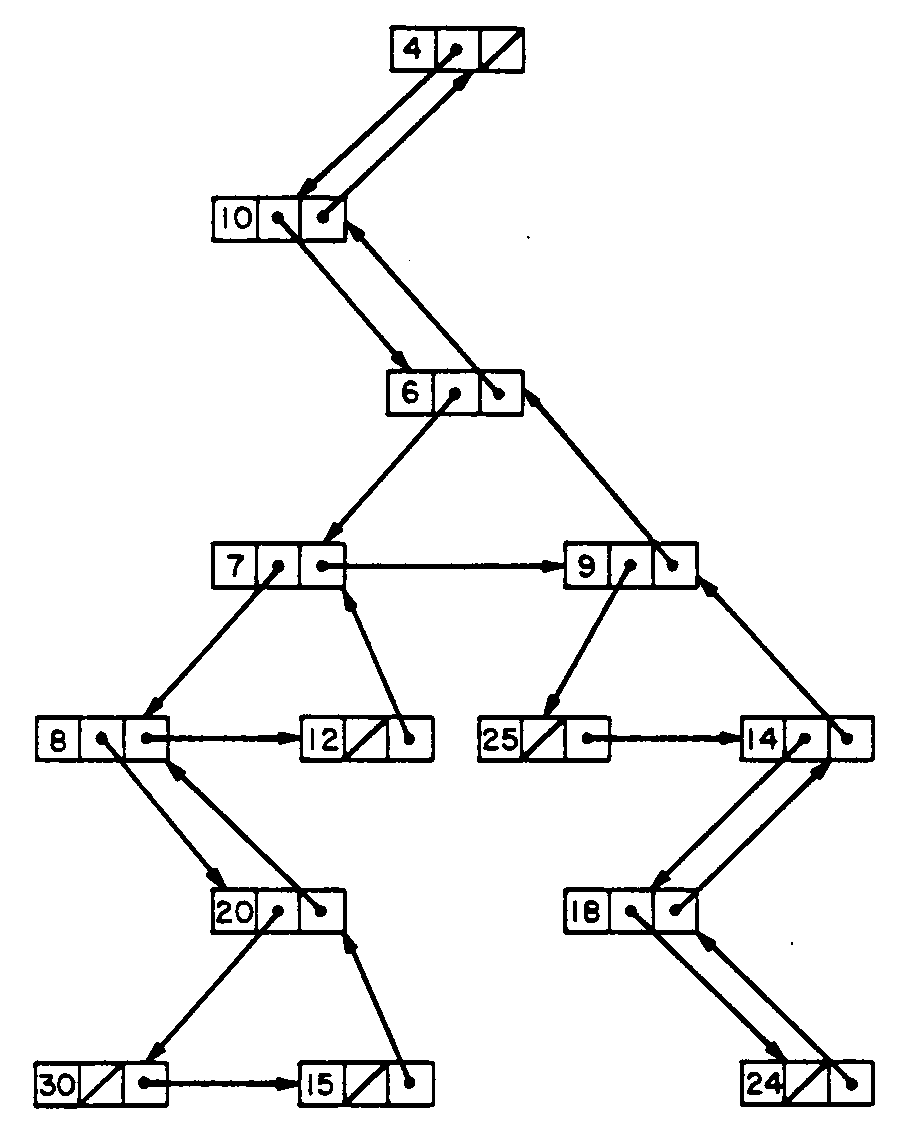
\includegraphics[height=7cm]{fig3.png}
\end{frame}

\begin{frame}
\frametitle{Child, sibling representation}

\begin{columns}[c]
\column{.5\textwidth}
Every node has a left pointer to its first child and a right pointer its next
sibling.\\

A parent pointer may be used in addition for more efficient
\textbf{decrease-key} and \textbf{delete} operations (constant factor).
\column{.5\textwidth}
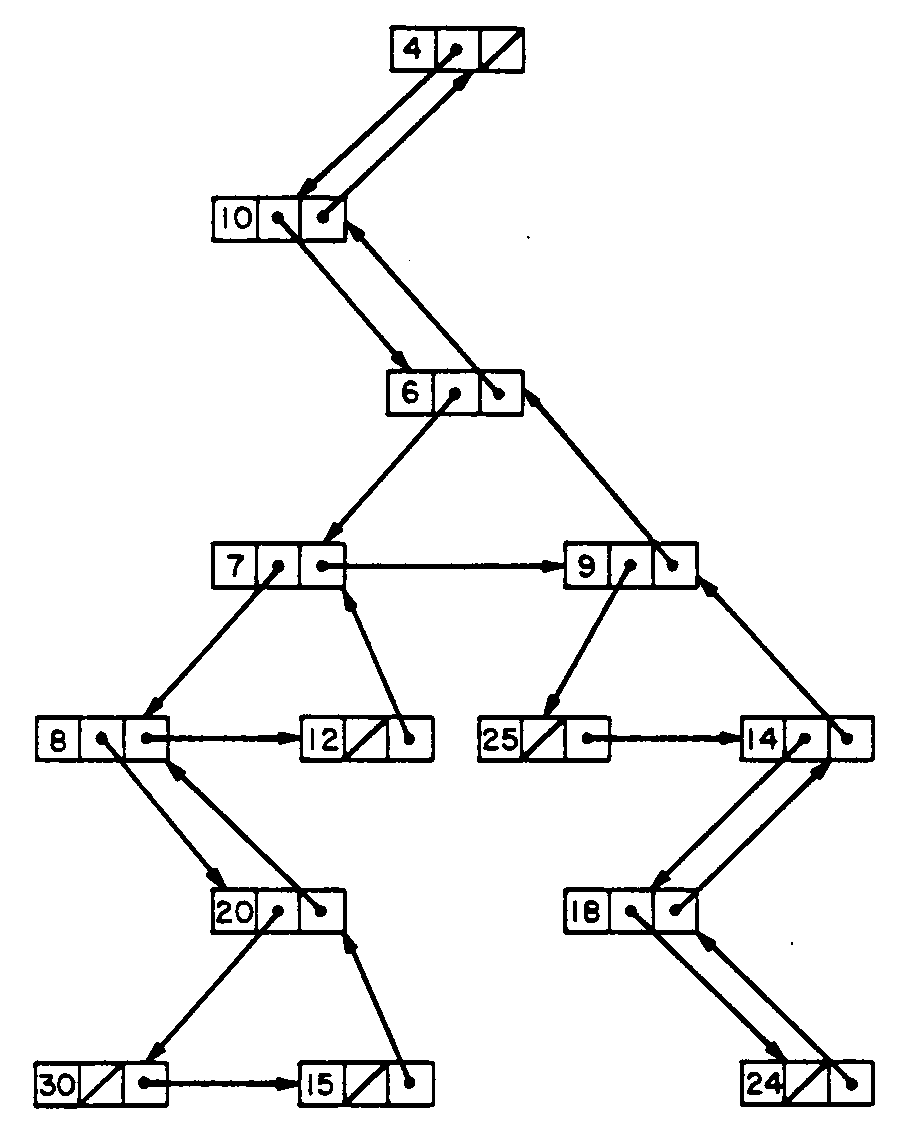
\includegraphics[height=5cm]{fig3.png}
\end{columns}

\end{frame}

\begin{frame}
\frametitle{Running times for the trivial operations}

\textbf{find-min}, \textbf{insert}, \textbf{meld} and \textbf{decrease-key} all
run in $O(1)$ time.

\textbf{delete-min} and \textbf{delete} are the only non-constant-time
operations.

\end{frame}

\begin{frame}
\frametitle{delete-min}

\begin{enumerate}
\item Remove tree root - $O(1)$ time
\item Link remaining heap-ordered trees - worst case $\Theta(n)$ time
\end{enumerate}

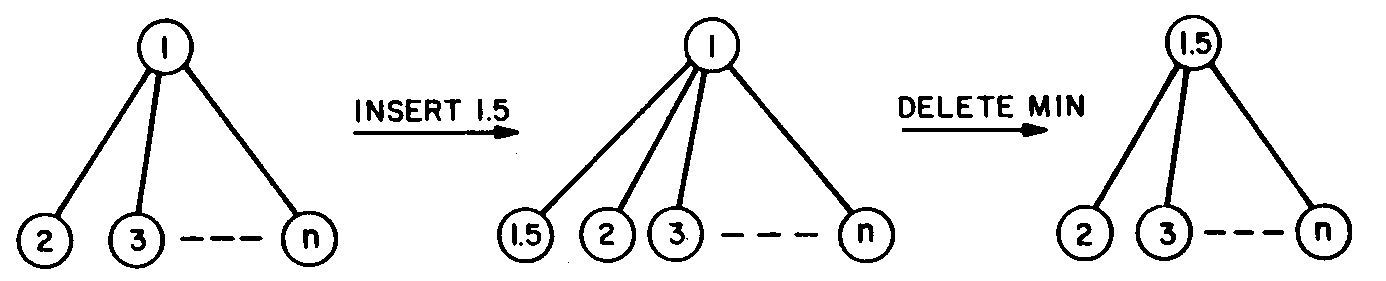
\includegraphics[width=10cm]{fig4.png}

Can be improved to $O(\log n)$ amortized time.

\end{frame}
 
\begin{frame}
\frametitle{Two-pass linking}

\begin{enumerate}
\item Link the trees in pairs (first pass)
\item Link a selected tree with the remaining paired trees (second pass)
\end{enumerate}

Can take $\Theta(\sqrt{n})$ amortized time depending on how the trees are paired
in the first pass.
\end{frame}
 
\begin{frame}
\frametitle{Two-pass linking}

$n = k(k+3)/2$: Pairing takes $\Omega(\sqrt{n})$ time.

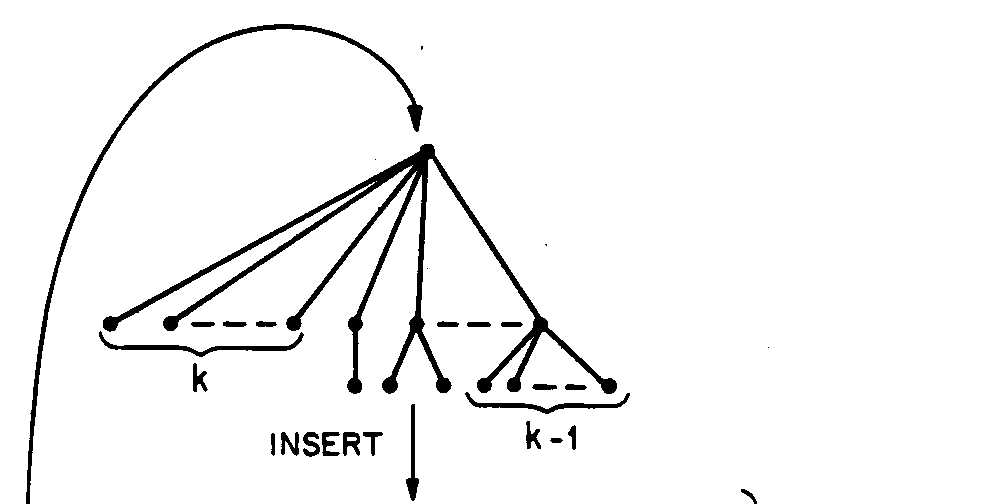
\includegraphics[width=10cm]{fig5-1.png}

\end{frame}
 
\begin{frame}
\frametitle{Two-pass linking}

$n = k(k+3)/2$: Pairing takes $\Omega(\sqrt{n})$ time.

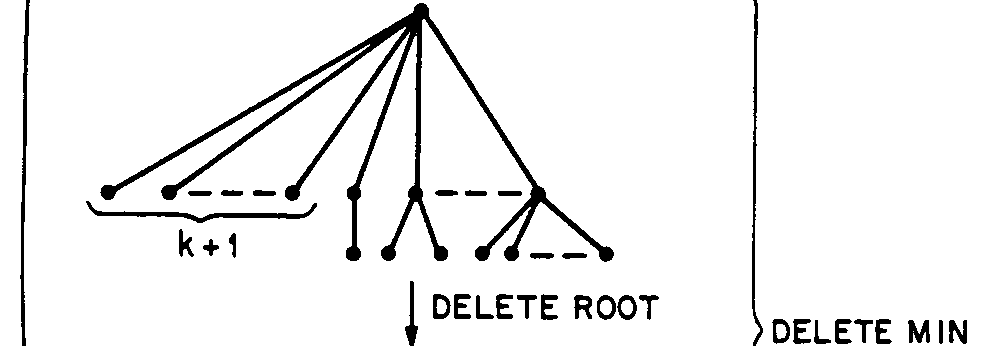
\includegraphics[width=10cm]{fig5-2.png}

\end{frame}
 
\begin{frame}
\frametitle{Two-pass linking}

$n = k(k+3)/2$: Pairing takes $\Omega(\sqrt{n})$ time.

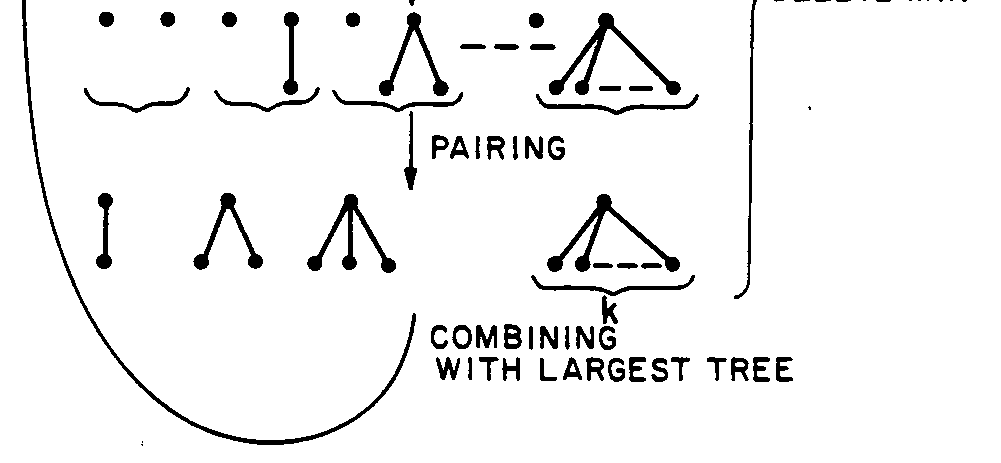
\includegraphics[width=10cm]{fig5-3.png}

\end{frame}
 
\begin{frame}
\frametitle{Two-pass linking: A better strategy}

\begin{enumerate}
\item Pair the trees in the order they were attached in the first place (1st and 2nd,
3rd and 4th etc.)

\item Link the paired trees in the opposite order (last-paired to first-paired).
\end{enumerate}
\end{frame}

\begin{frame}
\frametitle{Two-pass linking: A better strategy}

Pairing in-order:

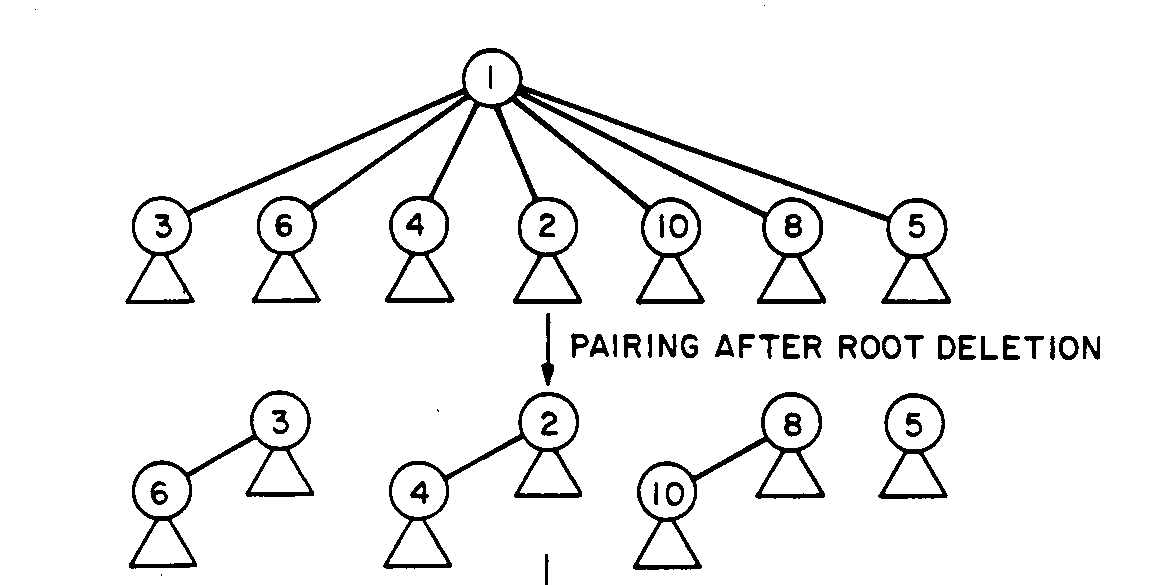
\includegraphics[width=10cm]{fig6-1.png}

\end{frame}

\begin{frame}
\frametitle{Two-pass linking: A better strategy}

Linking right-to-left:

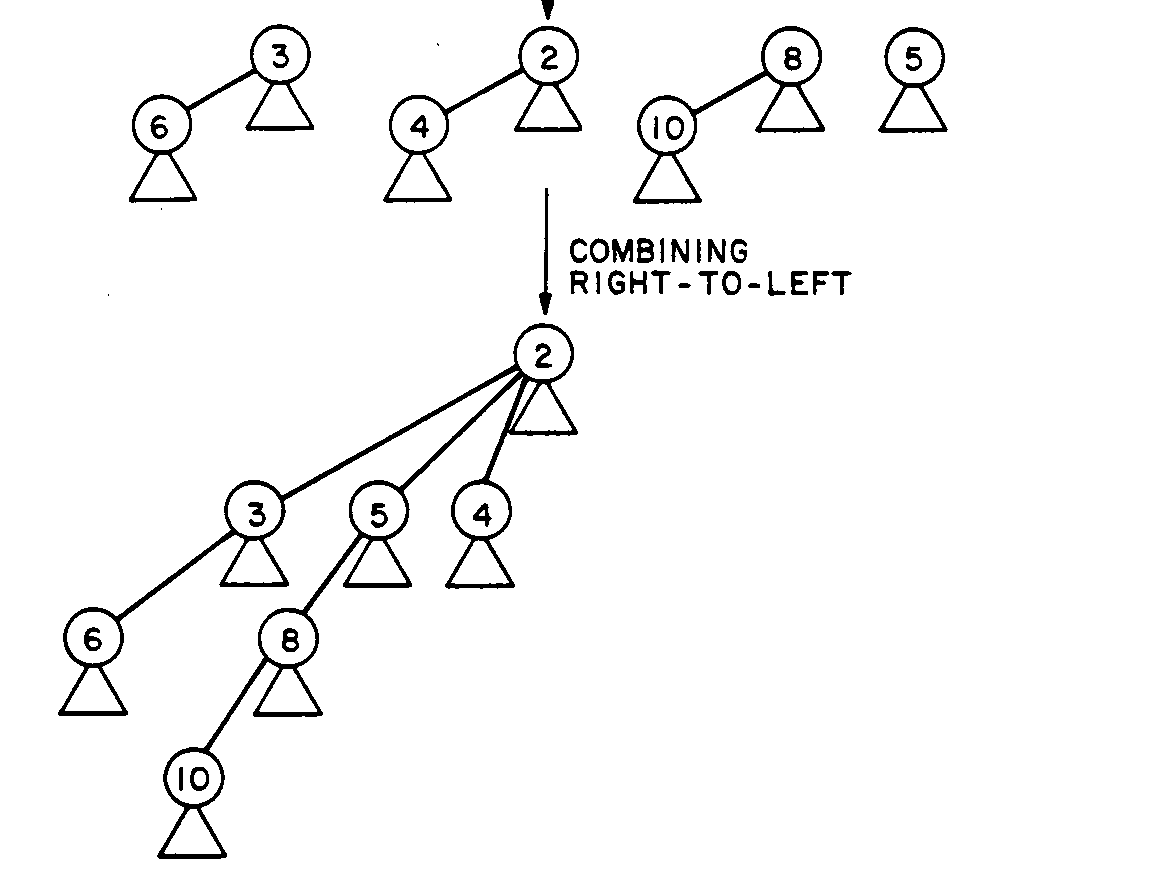
\includegraphics[width=10cm]{fig6-2.png}

\end{frame}

\begin{frame}
\frametitle{Amortized running times}

\textbf{Conjecture}: The various operations on pairing heaps have the following
amortized running times: $O(1)$ for \textbf{find-min}, \textbf{insert},
\textbf{meld} and \textbf{decrease-key}, and $O(\log n)$ for \textbf{delete-min}
and \textbf{delete}.

\vspace{\baselineskip}

Unable to be proven (at least in '86). Weaker result:

\vspace{\baselineskip}

\textbf{Theorem}: On pairing heaps, the operation \textbf{find-min} runs in
$O(1)$ amortized time, and the other operations run in $O(\log n)$ amortized
time.

\vspace{\baselineskip}

Since the effects of a \textbf{delete-min} operation yield close similarities to
a \textbf{splay} operation the proof is similar to the one for
\emph{self-adjusting search trees} using the same potential function.

\end{frame}

\begin{frame}
\frametitle{Variants}

\begin{enumerate}
\item Stasko-Vitter lazy insertion: Inserted elements are held in an auxiliary
buffer and melded into the heap when running \textbf{delete-min}. Improves
\textbf{insert} to $O(1)$ amortized time.

\item Elmasry Costless Meld: Decreased elements are added to a list of decreased
nodes and linked into the heap when running \textbf{delete-min} or when melding
two heaps (only for the smaller heap). Improves \textbf{decrease-key} to $O(\log
\log n)$ amortized cost and \textbf{meld} to zero amortized cost.
\end{enumerate}

\begin{figure}
\caption{Amortized running time, pairing heap variants}
\begin{tabular}{|c|c|c|c|c|} 
\hline
Original & $O(\log n)$ & $O(\log n)$ & $O(\log n)$ & $O(\log n)$ \\
\hline
Lazy insertion & $O(1)$ & $O(\log n)$ & $O(\log n)$ & $O(\log n)$ \\
\hline
Costless meld & $O(1)$ & $O(\log n)$ & $O(\log \log n)$ & zero \\
\hline
\end{tabular}
\end{figure}
\end{frame}

\end{document}
 
